\section{Contexto y trabajos realizados}

    Argentina continúa utilizando sistemas de enclavamiento mecánicos o electromecánicos de mediados dedl siglo XX [REF], mientras que otros países han actualizado sus sistemas de transporte de cargas y pasajeros con electrónica de última generación. La falta de mantenimiento adecuado y obsolesencia tecnológica impacta negativamente en la seguridad que dichos sistemas pueden brindar a los pasajeros, a la carga que transportan y/o a la infraestructura que utilizan.

    Adicionalmente, los sistemas de enclavamiento son en su totalidad importados y muy costosos, fabricados por una docena de empresas a nivel mundial, lo cual restringe la competencia y por lo tanto la variedad de precios es limitada. Un sistema de enclavamientos completo puede costar mas de 10 millones de dólares [REF], pero no se necesita solamente uno sino dececnas de ellos para modernizar toda la zona metropolitana de buenos Aires.

    En este contexto, en 2015 se creó el CONICET-GICSAFe [REF], cuyas siglas corresponden al Grupo de Investigación en Calidad y Seguridad de las Aplicaciones Ferroviarias, conformado por docentes e investigadores de una decena de universidades e instituciones públicas argentinas. El grupo desarrolla sistemas electrónicos e informáticos para aplicaciones ferroviarias relacionadas con la seguridad, a partir de la generación de un prototipo funcional y la documentación correspondiente que luego se transfiere en su totalidad a Trenes Argentinos [REF], que es la Sociedad del Estado que opera las líneas Roca, Sarmiento, Mitre, San Martín y Belgrano Sur, entre otras. En la Figura \ref{fig:contexto} se ilustran todos los logros e hitos alcanzados por GICSAFe y los objetivos a futuro desde 2018 hasta 2025.

    \begin{figure}[h]
        \centering
        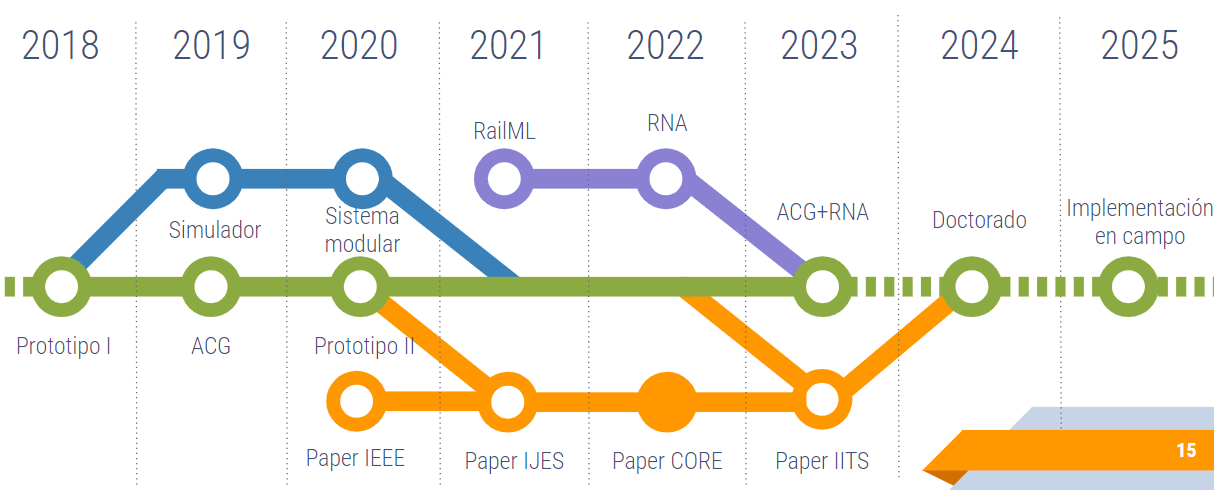
\includegraphics[width=1\textwidth]{Figuras/HojaDeRuta}
        \centering\caption{Trabajos realizados e hitos del proyecto.}
        \label{fig:contexto}
    \end{figure}

    En el año 2018 GICSAFe desarrolló un monitor de barreras ferroviarias instalado en la línea Roca, proyecto que ganó el premio Innnovar 2018 [REF] y permitió ganar experiencia en el área ferroviaria. Desde 2018 se tuvieron varias reuniones con diferentes funcionarios y profesionales de Trenes Argentinos. En particular, con la Gerencia de Ingeniería, Gerencia de Seguridad Operacional, Subgerencia de Desarrollo y Normas Técnicas, Subgerencia de Transporte, Gerencia de Señalamiento, entre otros, de los cuales surgió el interés en el desarrollo del presente proyecto. De dichas visitas y otras posteriores se obtuvo la totalidad de las fotografías incluidas en esta memoria. 

    En el marco de la Maestría de sistemas embebidos, culminada en 2020, se desarrollo un primer prototipo de sistema de enclavamiento con código generado automáticamente en base a un modelo de grafos. Los resultados fueron publicados en IEEE Latin American Transaction en 2020 y en International Journal of Embedded Systems en 2021. En simultáneo, el ingeniero Lucas Dórdolo, miembro de GICSAFe, presentó una actualización del sistema monitor de barreras: el sistema modular [REF], que permitió la lectura y transmisión de datos de la red ferroviaria en tiempo real. Adicionalmente, miembros de GICSAFe pertenecientes a UTN-Haedo comenzaron el desarrollo de un simulador de enclavamientos en tiempo real, que permitió resolver varias cuestiones técnicas de la implementación final del sistema de enclavamiento.

    Hacia finales de 2019 se iniciaron reuniones con miembros de la Comisión Nacional de Energía Atómica (CNEA), para integrar el proyecto en sus plataformas de hardware ampliamente testeada en el ámbito de los sistemas críticos. Además del intercambio de conocimientos y la puesta en común de estrategias a utilizar, se aprovechó todo lo posible la amplia experiencia que ellos brindaron a GICSAFe.
    
    A mediados de 2020, ya formalmente inscripto en el doctorado, se comenzó el desarrollo de una librería compatible con railML 3.0, lo cual se incorporó al primer analizador de redes ferroviarias en 2022, cuyos resultados se publicaron en IEEE Transactions on Intelligent Transportation Systems en 2023. La verificación y validación automática del sistema mediante métodos formales es parte del trabajo de doctorado del ingeniero Santiago Germino, iniciado en 2021. La integración de todas estas herramientas se aplicará en un sistema de enclavamientos a ser instalado en una playa de maniobras real en 2025. 